\chapter{Text classification}
Information extraction from the text can be stated as a text classification task.
Given a text, we want to assign a class it belongs to.
The class can be anything, from the text's category to the text's sentiment or the text's author's gender.
Depending on the number of classes, we can distinguish between \textbf{binary} (2) and \textbf{multiclass} (2+) classification.
We might want to classify the text by multiple labels; we thus also distinguish between \textbf{single-label}
and \textbf{multi-label} classification.


When considering what implicit information we wanted to extract, we focused on tasks
that are hard for humans to classify correctly. As was shown in \cite{wangDeepNeuralNetworks2017},
Deep Neural Networks (DNN) can achieve great results even on such tasks.
We thus narrowed down our research to the following four tasks:
\begin{enumerate}
    \item The category of the article
    \item Author's gender
    \item Day of week when the article was published
    \item News server where the article was published
\end{enumerate}
As a target language, we chose Czech.
We can therefore rephrase our research question as a single-label multiclass text classification of Czech News articles.
To avoid ambiguity, we will refer to a single news article text as a \textbf{document} going forward.

\section{Machine Learning}
Text classification is usually approached as a supervised learning task. Our work is no exception.
We thus need a dataset with labels for each document to create a model in this setting.
To our knowledge, no such dataset exists. We thus had to create a new one.
Dataset creation and its content will be described in the next chapter.

\section{Evaluation Metrics}
\label{sec:metrics}
To assess the model's performance, we need to define some metrics.
We start by defining metrics for binary classification and then extend them to multiclass classification.
In Binary classification, we have two classes; positive and negative. Thus we can have four possible outcomes:
\begin{enumerate}
    \item True positive(TP) - prediction postive, label positive
    \item True negative(TN) - prediction negative, label negative
    \item False negative(FN) - prediction negative, label positive
    \item False positive(FP) - prediction positive, label negative
\end{enumerate}

The most basic metric is accuracy, which is defined as
\begin{equation}
    \label{eq:accuracy}
    \text{Accuracy} = \frac{TP + TN}{TP + TN + FP + FN}
\end{equation}
However, accuracy often fails to capture the whole picture.
Let's consider a dataset of 1000 people, where 990 are healthy and ten are sick.
Such a dataset is called imbalanced, as the number of classes is distributed unequally.
On this dataset, we could achieve 99\% accuracy by always predicting that the person is healthy.
Such a model would be useless in practice, as it could not detect sick people.

\subsection{Precision and Recall}
Precision and recall deal with the issue of imbalanced datasets.
They are defined as
\begin{equation}
    \label{eq:precision}
    \text{Precision} = \frac{TP}{TP + FP}
\end{equation}
\begin{equation}
    \label{eq:recall}
    \text{Recall} = \frac{TP}{TP + FN}
\end{equation}
Considering the same model as before, we will score 0\% recall and 100\% precision\todo{Not sure about this}.
If we were to increase the recall by always predicting sick, we would achieve 100\% recall and 10\% precision.
A good model should thus have both high precision and recall.

\subsection{F1 Score}
The $F_{\beta}$ score is the answer to our requirements.
It combines precision and recall into one metric, and is defined as
\begin{equation}
    \label{eq:f1}
    F_{\beta} = (1 + \beta^2) \cdot \frac{\text{Precision} \cdot \text{Recall}}{\beta^2 \cdot \text{Precision} + \text{Recall}}
\end{equation}

\subsection{Extending to multiclass - Micro and Macro Averaging}
We can use micro and macro averaging to extend the binary metrics to a multiclass case.
In the case of micro averaging, we consider $TP$, $TN$, $FP$, and $FN$ as the sum of respective values for each class.
We then calculate the metrics as before.
In the case of macro averaging, we calculate the metrics for each class and then average them.
This results in treating each class equally irregardless of the number of samples in each class.

\section{Notation intermezzo}
\label{sec:notation}
Going forward we will use the following notation:
\begin{itemize}
    \item non-bold lowercase letters (e.g. $x$) will denote a scalar
    \item bold lowercase letters (e.g. $\mathbf{x}$) will denote a vector
    \item bold uppercase letters (e.g. $\mathbf{X}$) will denote a matrix
    \item letters with hat (e.g. $\hat{x}$) will denote a predicted value
    \item $|V|$ will denote size of set $V$
\end{itemize}
All vectors are column vectors unless otherwise stated.

\section{Document Representation}
\label{sec:representation}
To train a model, we need to represent the document in a way that the model can understand.
Let's consider a dataset $D$ of $N$ documents. We can use the following representations:

\subsection{Bag of Words(BOW)}
\label{sec:bow}
One way to represent the document is to encode each word based on the number of occurrences in the document.
Such is an idea of the Bag of Words encoding. To obtain a BOW representation, we do the following:
\begin{enumerate}
    \item Tokenize the dataset. This is a process of splitting the text into smaller units called tokens (usually words).
    \item Create a vocabulary $V$ of all the tokens in the dataset.
    \item Represent document $d$ as vector of weights $(C_{d}^1, C_{d}^2, \dots, C_{d}^{|V|})$ where $C_{d}^i$
    is the number of occurrences of token $i$ in document $d$.
\end{enumerate}
This representation allows us to store the BOW representation of the dataset as a sparse $N \times |V|$ matrix,

\subsection{TF-IDF}
\label{sec:tfidf}
TF-IDF is an extension of the BOW representation, where we also consider the document's token frequency.
To represent the weight of token $t$ in document $d$, we use the following formula:
\begin{equation}
    \label{eq:tfidf}
    \text{TF-IDF}(t, d) = \text{TF}(t, d) \cdot \text{IDF}(t)
\end{equation}
where TF and IDF are defined as
\begin{equation}
    \label{eq:tf}
    \text{TF}(t, d) = \frac{C_{d}^t}{|d|}
\end{equation}
\begin{equation}
    \label{eq:idf}
    \text{IDF}(t) = \log \frac{|D|}{\sum_{d \in D} (C_{d}^t)}
\end{equation}


\subsection{Subword Representations}
    The problem with preceding representations is that they cannot capture unseen words and require
    a large vocabulary. To solve this problem, we can use subword representations. Unlike the previous
    representations, subword representations are not fixed-sized.

    \subsubsection{Byte Pair Encoding (BPE)}
    \label{sec:bpe}
    Popularized by \cite{sennrichNeuralMachineTranslation2016b} algorithm is following:
    \begin{enumerate}
        \item Split sentences into words by whitespace and punctuation.
        \item Split each word into a single character and add the special end of the word token.
        \item Initializes the vocabulary with all the found characters and the end of the word token.
        \item Iteratively merge the most frequent pair of characters into a single character.
        \item Stop when the vocabulary size reaches the desired size.
    \end{enumerate}
    We then use the vocabulary to encode the document as a sequence of token ids.

    \subsubsection{WordPiece}
    \label{sec:wordpiece}
    WordPiece is a modification of BPE that uses a different merging
    strategy and pre-tokenization. It was first introduced by \cite{schusterJapaneseKoreanVoice2012}
    and improved by \cite{wuGoogleNeuralMachine2016}.
    For pre-tokenization, it adds a special token at the beginning instead of the end of the word.
    As for the merging strategy, we choose the pair that maximizes the likelihood of the training data when merged.

    \subsubsection{SentencePiece (SPM)}
    \label{sec:spm}
    Introduced by \cite{kudoSentencePieceSimpleLanguage2018}, SPM is rather a modular tokenizer than an algorithm.
    It unifies the preprocessing and tokenization steps and allows different sub-word algorithms to be used.
    Among other things, it also addresses the problem of multiple space characters encoding, which is not possible in the above sub-word algorithms.
    It does so by introducing a special token for the space character.


    \subsection{Byte Pair Encoding (BBPE)}
    \label{sec:bbpe}
    BBPE is a modification of BPE. Instead of considering single characters we consider single bytes.
    This ensures that we can encode any character.

\section{ML Models}
\label{sec:models}
This section reviews the ML models we will use in experiments.
Our intention is not to provide a comprehensive review of text classification approaches.
If the reader is interested in such a work, we recommend \cite{kowsariTextClassificationAlgorithms2019}.
Note that we will not review Convolutional Neural Networks(CNN) or Recurrent Neural Networks(RNN).
However, we will refer to them and expect the reader to know them.

\subsection{Multinomial Logistic Regression}
\label{sec:mlr}
Multinomial Logistic regression (MLR) is a simple linear model.
The MLR with $k$ classes is represented by matrix of weights $\mathbf{W} \in R^{k, d} = (\mathbf{w_1}, \mathbf{w_2}, \dots \mathbf{w_n})^T$
and vector of biases $\mathbf{b} = (\beta_1, \beta_2, \dots \beta_k)$.

Given input $\mathbf{x} \in R^{d}$, with correct class $y == C_t$ the probability of model predicting class $C_i$ is given by
\begin{align}
    %% Softmax
    \sigma(\mathbf{z}) &= \frac{e^{z_i}}{\sum_{j=1}^{k} e^{z_j}} \\
    %% Probability
    P(C_i | \mathbf{x}; \mathbf{W}, \mathbf{b}) &= \sigma(\mathbf{W} \mathbf{x} + \mathbf{b})
\end{align}
The optimized loss function is cross-entropy loss:
\begin{equation}
    \mathcal{L}(\mathbf{x};\mathbf{W}, \mathbf{b}) = \log P(C_t \mathbf{x}; \mathbf{W}, \mathbf{b})
\end{equation}
 
The model is very simple, so it can't capture complex relationships between features.
However, it serves as a good baseline model, and unlike later models, it can be easily interpreted.

\subsection{Transformers}
\label{sec:transformers}
Transformers have been first proposed for a task of machine translation by \cite{vaswaniAttentionAllYou2017d}.
They have since become a state-of-the-art model for many NLP tasks, including Text Classification.
The original paper suggested using encoder-decoder architecture due to the nature of the machine translation task.
However, for text classification, there is no need for the decoder. Thus, the architecture can be simplified to only the encoder.
In the following sections by \textbf{transformer}, we will refer to the encoder part of the architecture.

\subsubsection{Architecture}
%import pdf
\begin{figure}[h]
    \centering
    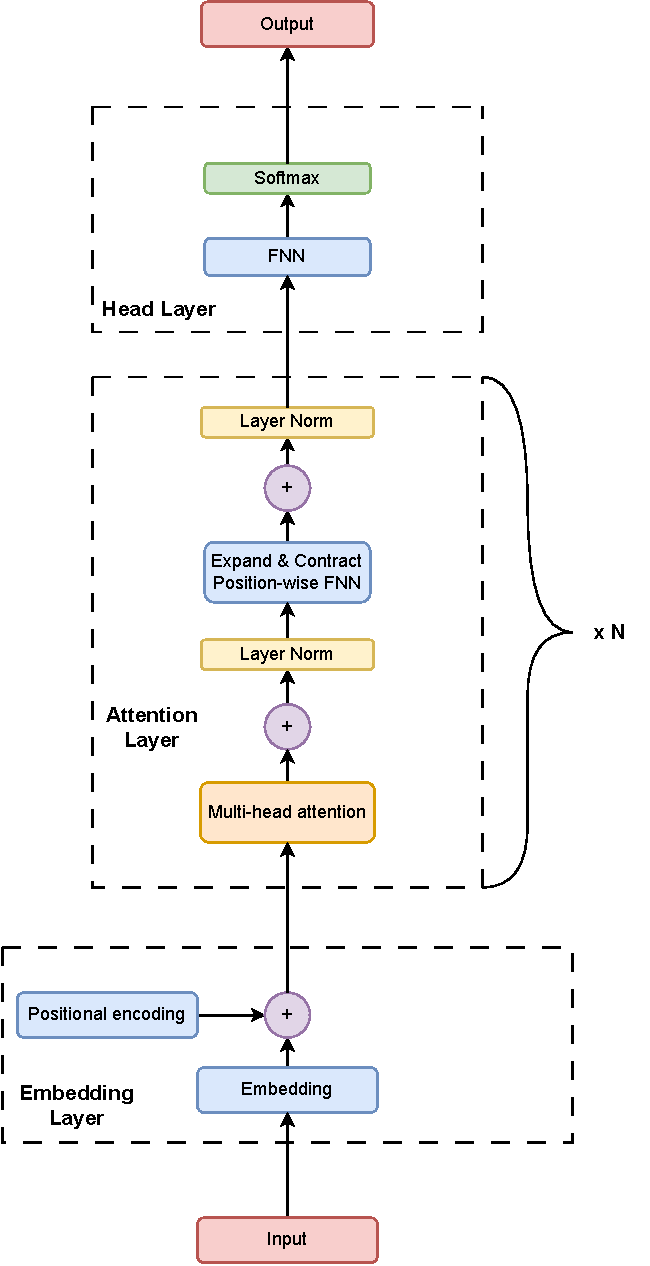
\includegraphics[width=0.7\linewidth]{img/transformer/trans_architecture.pdf}
    \caption{Transformer architecture, we omitted Dropout blocks for clarity.}
    \label{fig:transformer}
\end{figure}
    
The architecture of the transformer can be seen at \autoref{fig:transformer}.
The key components are:
\begin{itemize}
    \item Embedding layer
    \item Multi-Head Attention Block
    \item Head layer
\end{itemize}
We will now describe each of them in detail.
\subsubsection{Embedding Layer}
The first layer of the transformer is an embedding layer, it takes the input text encoded as a vector $\mathbf{x} \in R^{n}$,
where $n$ is the length of the input, with values in the range $[0, V)$, where $V$ is the vocabulary size.
The embedding layer embeds each vector element into vector space by employing a learnable matrix $\mathbf{E} \in R^{V, d}$, where $d$ is the arbitrary embedding dimension.
To encode the position of the word in the sentence, we add a learnable positional embedding $\mathbf{P} \in R^{n, d}$.
Thus the output of the embedding layer is given by:
\begin{equation}
    \mathbf{O} = OneHot(\mathbf{x}) \times \mathbf{E} + \mathbf{P}
\end{equation}
where $OneHot(\mathbf{x})$ is a matrix of one-hot vectors, where each row corresponds to the one-hot vector of the corresponding element in $\mathbf{x}$.
This makes the model only accept fixed-length inputs.
\footnote{The original paper allowed for variable length inputs, by employing a different strategy for positional encoding.}

\subsubsection{Self-attention}
Self-attention is a key mechanism of transformer architecture.
The Queries (Q), Keys (K), and Values (V) matrices are computed from inputs as follows:
\begin{align}
    \mathbf{Q} &= \mathbf{X} \mathbf{W_q} \\
    \mathbf{K} &= \mathbf{X} \mathbf{W_k} \\
    \mathbf{V} &= \mathbf{X} \mathbf{W_v} \\
    \text{where } \mathbf{W_q}, \mathbf{W_k}, \mathbf{W_v} &\in R^{d, d} \text{are trainable matrices}
\end{align}
The output of the self-attention layer is then computed as follows:
\begin{align}
    \mathbf{O} &= \text{softmax}(\frac{\mathbf{Q} \mathbf{K}^T}{\sqrt{d}}) \mathbf{V} \\
    \label{eq:attention}
\end{align}
\footnote{The dimension hidden state of self-attention can be different from the embedding dimension. We use the same for simplicity}
The intuition behind the self-attention is that by doing a scalar product between query and key vectors,
the model learns to focus on the most relevant parts of the input.
Such parts will then have the highest weight in the output in values multiplication.

\subsubsection{Masked Self-attention}
In many tasks, we would like to configure which parts of the input can attend to which parts of the input.
This is achieved by masking the attention matrix before applying softmax at \autoref{eq:attention} in first attention layer.

\subsubsection{Multihead attention}
The multi-head attention is an extension of self-attention.
Instead of doing just one attention, we do multiple attention in parallel, every attention with different Query, Key and Value matrices.
The outputs are then concatenated and passed through a linear layer.

\subsubsection{Head Layer}
Head Layer is task-dependent and the server converts the output of the transformer to the desired output.

\subsection{Benefits and Drawbacks}
\label{sec:benefits-and-drawbacks}
What transformers mostly improved were two things:
\begin{itemize}
    \item Capturing of long-range dependencies.
    \item Parallelization of the model. Unlike RNNs, we don't process a single input at a time,
    but all of them in parallel. This allows for much faster training.
\end{itemize}
However, advantages haven't come without a cost. One of the biggest problems with transformers
is their memory complexity. The self-attention layer requires $O(n^2)$ memory and $O(d \times n^2)$ time complexity.
This limits the use of transformers to lower-length inputs. However, there has been
a lot of work done in recent years to mitigate this issue.
\cite{zhuangSurveyEfficientTraining2023} surveys the most popular methods,
\cite{wuMEMORIZINGTRANSFORMERS2022}, proposes a novel method for memory-efficient long-range attention using k-NN.

\subsection{Transfer Learning}
\label{sec:transfer-learning}
Transfer learning is a technique that allows using of knowledge gained from one task to solve another.
The popular method of transfer learning is fine-tuning. To fine-tune a model we take a pre-trained model (\textbf{backbone})
and train it on a new task with a new task-specific head.

\subsection{Language Model}
The popular backbone models are language models (\textbf{LM}s). The goal of the LM is to predict the next token in a sentence.
Due to the simplicity of the task, can be trained in an unsupervised manner allowing for large-scale training.
The approach is fairly old and was used even before the transformers with RNNs
in \cite{daiSemisupervisedSequenceLearning2015} and \cite{petersSemisupervisedSequenceTagging2017}.
The transformers allowed this method to scale to much larger datasets and models.

\subsection{BERT}
\textbf{Bert}, introduced in \cite{devlinBERTPretrainingDeep2019a}, is a successor to the previous attempts of training transformers LMs, namely ELMo~(\cite{petersDeepContextualizedWord2018}) and GPT~(\cite{howardUniversalLanguageModel2018a}).
The main difference between BERT and previous methods is that it uses a bi-directional encoder.
Previous work used a single-direction encoder; LM model attending to either the left or the right context only.
The bi-directional encoder allows the model to attend to the context in both directions.
That's achieved by the Masked LM optimization objective.

\subsubsection{Masked LM}
\label{sec:masked-lm}
The goal of the masked LM is to predict the masked tokens in the text.
Taking input tokens and replacing some of them with a special token "[MASK]", the model is trained to predict the masked words.
As the model won't see the mask tokens during inference, some tokens in the input are replaced with random tokens from the vocabulary instead of the mask token.

\subsubsection{Next Sentence Prediction (NSP)}
The goal of the next sentence prediction is to predict if the two token sequences are consecutive in the original text.

\subsubsection{Input Representation}
The BERT uses a WordPiece tokenization \cite{wuGoogleNeuralMachine2016} to convert the input text to tokens.
Apart from learned tokens, BERT introduces three special tokens:
\begin{enumerate}
    \item \textbf{[CLS]} - Token appended to start of token sequence. The predicted output is based on the hidden state of this token.
    \item \textbf{[SEP]} - The token that is appended to the end of the token sequence.
    \item \textbf{[MASK]} - The token that is used for masking in \autoref{sec:masked-lm}.
\end{enumerate}


\subsubsection{Bert-base and Bert-large}
Bert model exists in two versions: BERT-base and BERT-large, they differ by the number of layers and hidden layer size.
\begin{table}[h]
    \centering\footnotesize\sf
    \begin{tabular}{lll}
        \toprule
        {} BERT-base & BERT-large \\
        \midrule
        hidden size & 768 & 1024 \\
        number of layers & 12 & 24 \\
        number of attention heads & 12 & 16 \\
        \bottomrule
    \end{tabular}
    \caption{Comparison of BERT-base and BERT-large}
    \label{tab:bert-base-large}
\end{table}


\subsection{RoBERTa}
\textbf{RoBERTa} introduced by \cite{liuRoBERTaRobustlyOptimized2019} is a further refinement of the BERT model.
It doesn't change the architecture of the model but instead changes the way the model is trained.
The key differences are displayed in \autoref{tab:bert-roberta}.
\begin{table}[h]
    \centering\footnotesize\sf
    \begin{tabular}{lll}
        \toprule
        {} BERT & RoBERTa \\
        \midrule
        batch size & 256 & 512 \\
        sequence length & 128 tokens 90\% and 512 tokens $10\%$ (BERT) \\
        tokenization & WordPiece & BPE \\
        data & 16GB & 160GB \\
        objective & Masked LM + NSP & Masked LM \\
        \bottomrule
    \end{tabular}
    \caption{Comparison of BERT and RoBERTa}
    \label{tab:bert-roberta}
\end{table}

\subsection{GPT-3}
\textbf{GPT-3} is a family of models introduced by \cite{brownLanguageModelsAre2020b}.
Due to them being developed by \textbf{OpenAI}\footnote{\url{https://openai.com/}}, they are not publicly available and not much is known about them.
As per \cite{brownLanguageModelsAre2020b}, the GPT-3 models are transformer-based LMs with parameters ranging from 125M to 175B, trained on
a large multilingual dataset with more than 570GB of text. The tokenizer is based on the BBPE modification described in \cite{radfordLanguageModelsArea}.
To solve efficiency issues described in \autoref{sec:benefits-and-drawbacks}, the model also employs sparse attention modification described in \cite{childGeneratingLongSequences2019}.

The OpenAI offers paid finetuning and inference of the derivatives of GPT-3 models but no information about the models themselves.

\subsection{Multi-linguality of LMs}
\label{sec:multilinguality}
Both BERT and RoBERTa are trained on exclusively English data. To allow extension to other languages,
multi-lingual models were introduced. Namely, XLM (\cite{lampleCrosslingualLanguageModel2019}), XML-R (\cite{conneauUnsupervisedCrosslingualRepresentation2020})
and m-BERT \todo{I CANT FIND THE PAPER AAAAAA}. GPT-3 models could also be considered a multilingual model as $7\%$ of the training data is in non-English languages
and show great results on translation tasks to English.

While the models have shown multi-lingual capabilities,
they possess two major drawbacks:
\begin{itemize}
    \item To accompany a large variety of languages the dictionary thus the embedding layer is very large.
    \item Length of tokenized sequences tends to be very long, due to multi-lingual tokenization training.
\end{itemize}
It has been also shown by \cite{strakaRobeCzechCzechRoBERTa2021} and \cite{scheibleGottBERTPureGerman2020} that the
mono-lingual models can still outperform the multi-lingual models on certain target language tasks while being significantly smaller.

\subsection{Czech Mono-lingual LM Models}
    \begin{table}[h]
    \centering\footnotesize\sf
    \begin{tabular}{|l|l|l|l|l|}
    \toprule
    Model & Base Model & Tokenizer & Training Data & \# Params \\
    \midrule
    M-BERT \cite{devlinBERTPretrainingDeep2019a} & BERT-base & WordPiece & 120k Wiki, 104 langs & 179M \\
    XLM-RoBERTa-base \cite{conneauUnsupervisedCrosslingualRepresentation2020} & RoBERTa-base & SPM & 250k CC, 100 langs (2TB) & 278M \\
    XLM-RoBERTa-large \cite{conneauUnsupervisedCrosslingualRepresentation2020} & RoBERTa-large & SPM & 250k CC, 100 langs (2TB) & 560M \\
    \midrule
    Czert \cite{sidoCzertCzechBERTlike2021} & BERT-base & WordPiece & 40k Nat+Wiki+News (37GB) & 110M \\
    RobeCzech \cite{strakaRobeCzechCzechRoBERTa2021} & RoBERTa-base & BBPE & 52k Nat+Wiki+Czes+W2C & 126M \\
    FERNET-C5 \cite{leheckaComparisonCzechTransformers2021} & BERT-base & SPM & 100k C5 (93GB) & 164M \\
    FERNET-News \cite{leheckaComparisonCzechTransformers2021} & RoBERTa-base & BBPE & 50k News Corpus (21GB) & 124M \\
    Small-E-Czech \cite{kocianSiameseBERTbasedModel2021} & Electra-base & WordPiece & Seznam.cz in-house Czech corpus (253GB) & 13 M \\
    \bottomrule
    \end{tabular}
    \caption{Table comparing Multi-lingual and Czech monolingual models.
        Electra-base (\cite{clarkELECTRAPretrainingText2020}) is transformer architecture trained 
        with discriminative pre-training rather than generative.
        Table is slightly modified version from \cite{leheckaComparisonCzechTransformers2021}}
    \label{tab:czech-monolingual}
    \end{table}
    Czech pre-trained LM models are depicted in \autoref{tab:czech-monolingual} \todo{Is it ok to use their table?}.
    We highlight \textbf{FERNET-News} and \textbf{RobeCzech} as they will be used in experiments.
    \todo{Should I add something about the models? Most important data are in the table so idk}